\section*{Datenbank}

Gegen ist eine Datenbank mit folgenden Tabellenschemata:  \\\\

Freizeitpark(\underline{id:INT}, name:STRING, \dotuline{gemeindeschluessel:STRING}, strasse:STRING, url:STRING, breitengrad:FLOAT, laengengrad:FLOAT)\\

Gemeinde(\underline{schluessel:STRING}, regierungsbezirk:STRING, kreis:STRING, name:STRING, zusatz:STRING, plz:STRING, flaeche:FLOAT, einwohner\_m:INT, einwohner\_w:INT)\\

Nachbargemeinde(\dotuline{gemeindeschluessel\_1:STRING}, \dotuline{gemeindeschluessel\_2:STRING})\\

Radweg(name:STRING, \underline{radweg\_id:STRING})\\

Radweg\_zu\_Gemeinde(\dotuline{radweg\_id:STRING}, \dotuline{gemeindeschluessel:STRING})\\

Schwimmbad(\underline{id:INT}, name:STRING, art:STRING, \dotuline{gemeindeschluessel:STRING}, strasse:STRING, url:STRING, breitengrad:FLOAT, laengengrad:FLOAT)\\

Wanderweg(name:STRING, \underline{wanderweg\_id:STRING})\\

Wanderweg\_zu\_Gemeinde(\dotuline{wanderweg\_id:STRING}, \dotuline{gemeindeschluessel:STRING})\\

Zoo(\underline{id:INT}, name:STRING, \dotuline{gemeindeschluessel:STRING}, strasse:STRING, url:STRING, breitengrad:FLOAT, laengengrad:FLOAT)\\


\section*{Aufgabe 1}







\begin{minipage}[t]{\textwidth}
Schreibe eine SQL-Abfrage, die die Namen aller Zoos in einer Gemeinde namens "Erlangen" ausgibt.

\LoesungLine{SELECT Zoo.name\\
FROM Zoo,Gemeinde\\
WHERE Zoo.gemeindeschluessel = Gemeinde.schluessel\\
AND Gemeinde.name="Erlangen"}{4}
\end{minipage}


\vspace{0.3cm}

Schreibe eine SQL-Abfrage, die die Anzahl an Radwegen, die an Gemeinden im PLZ-Bereich \emphOrange{größer} als 96400 angrenzen, ausgibt.

\LoesungLine{SELECT COUNT(*)\\
FROM Gemeinde, Radweg\_zu\_Gemeinde\\
WHERE Gemeinde.schluessel=Radweg\_zu\_Gemeinde.gemeindeschluessel\\
  AND Gemeinde.plz > 96400}{4}




\begin{minipage}[t]{\textwidth}
\section*{Aufgabe 2}

Zeichne das vollständige (Datentypen, Beziehungen, Kardinalitäten, alle Klassen) Klassendiagramm für diese Datenbank.


\LoesungKaro{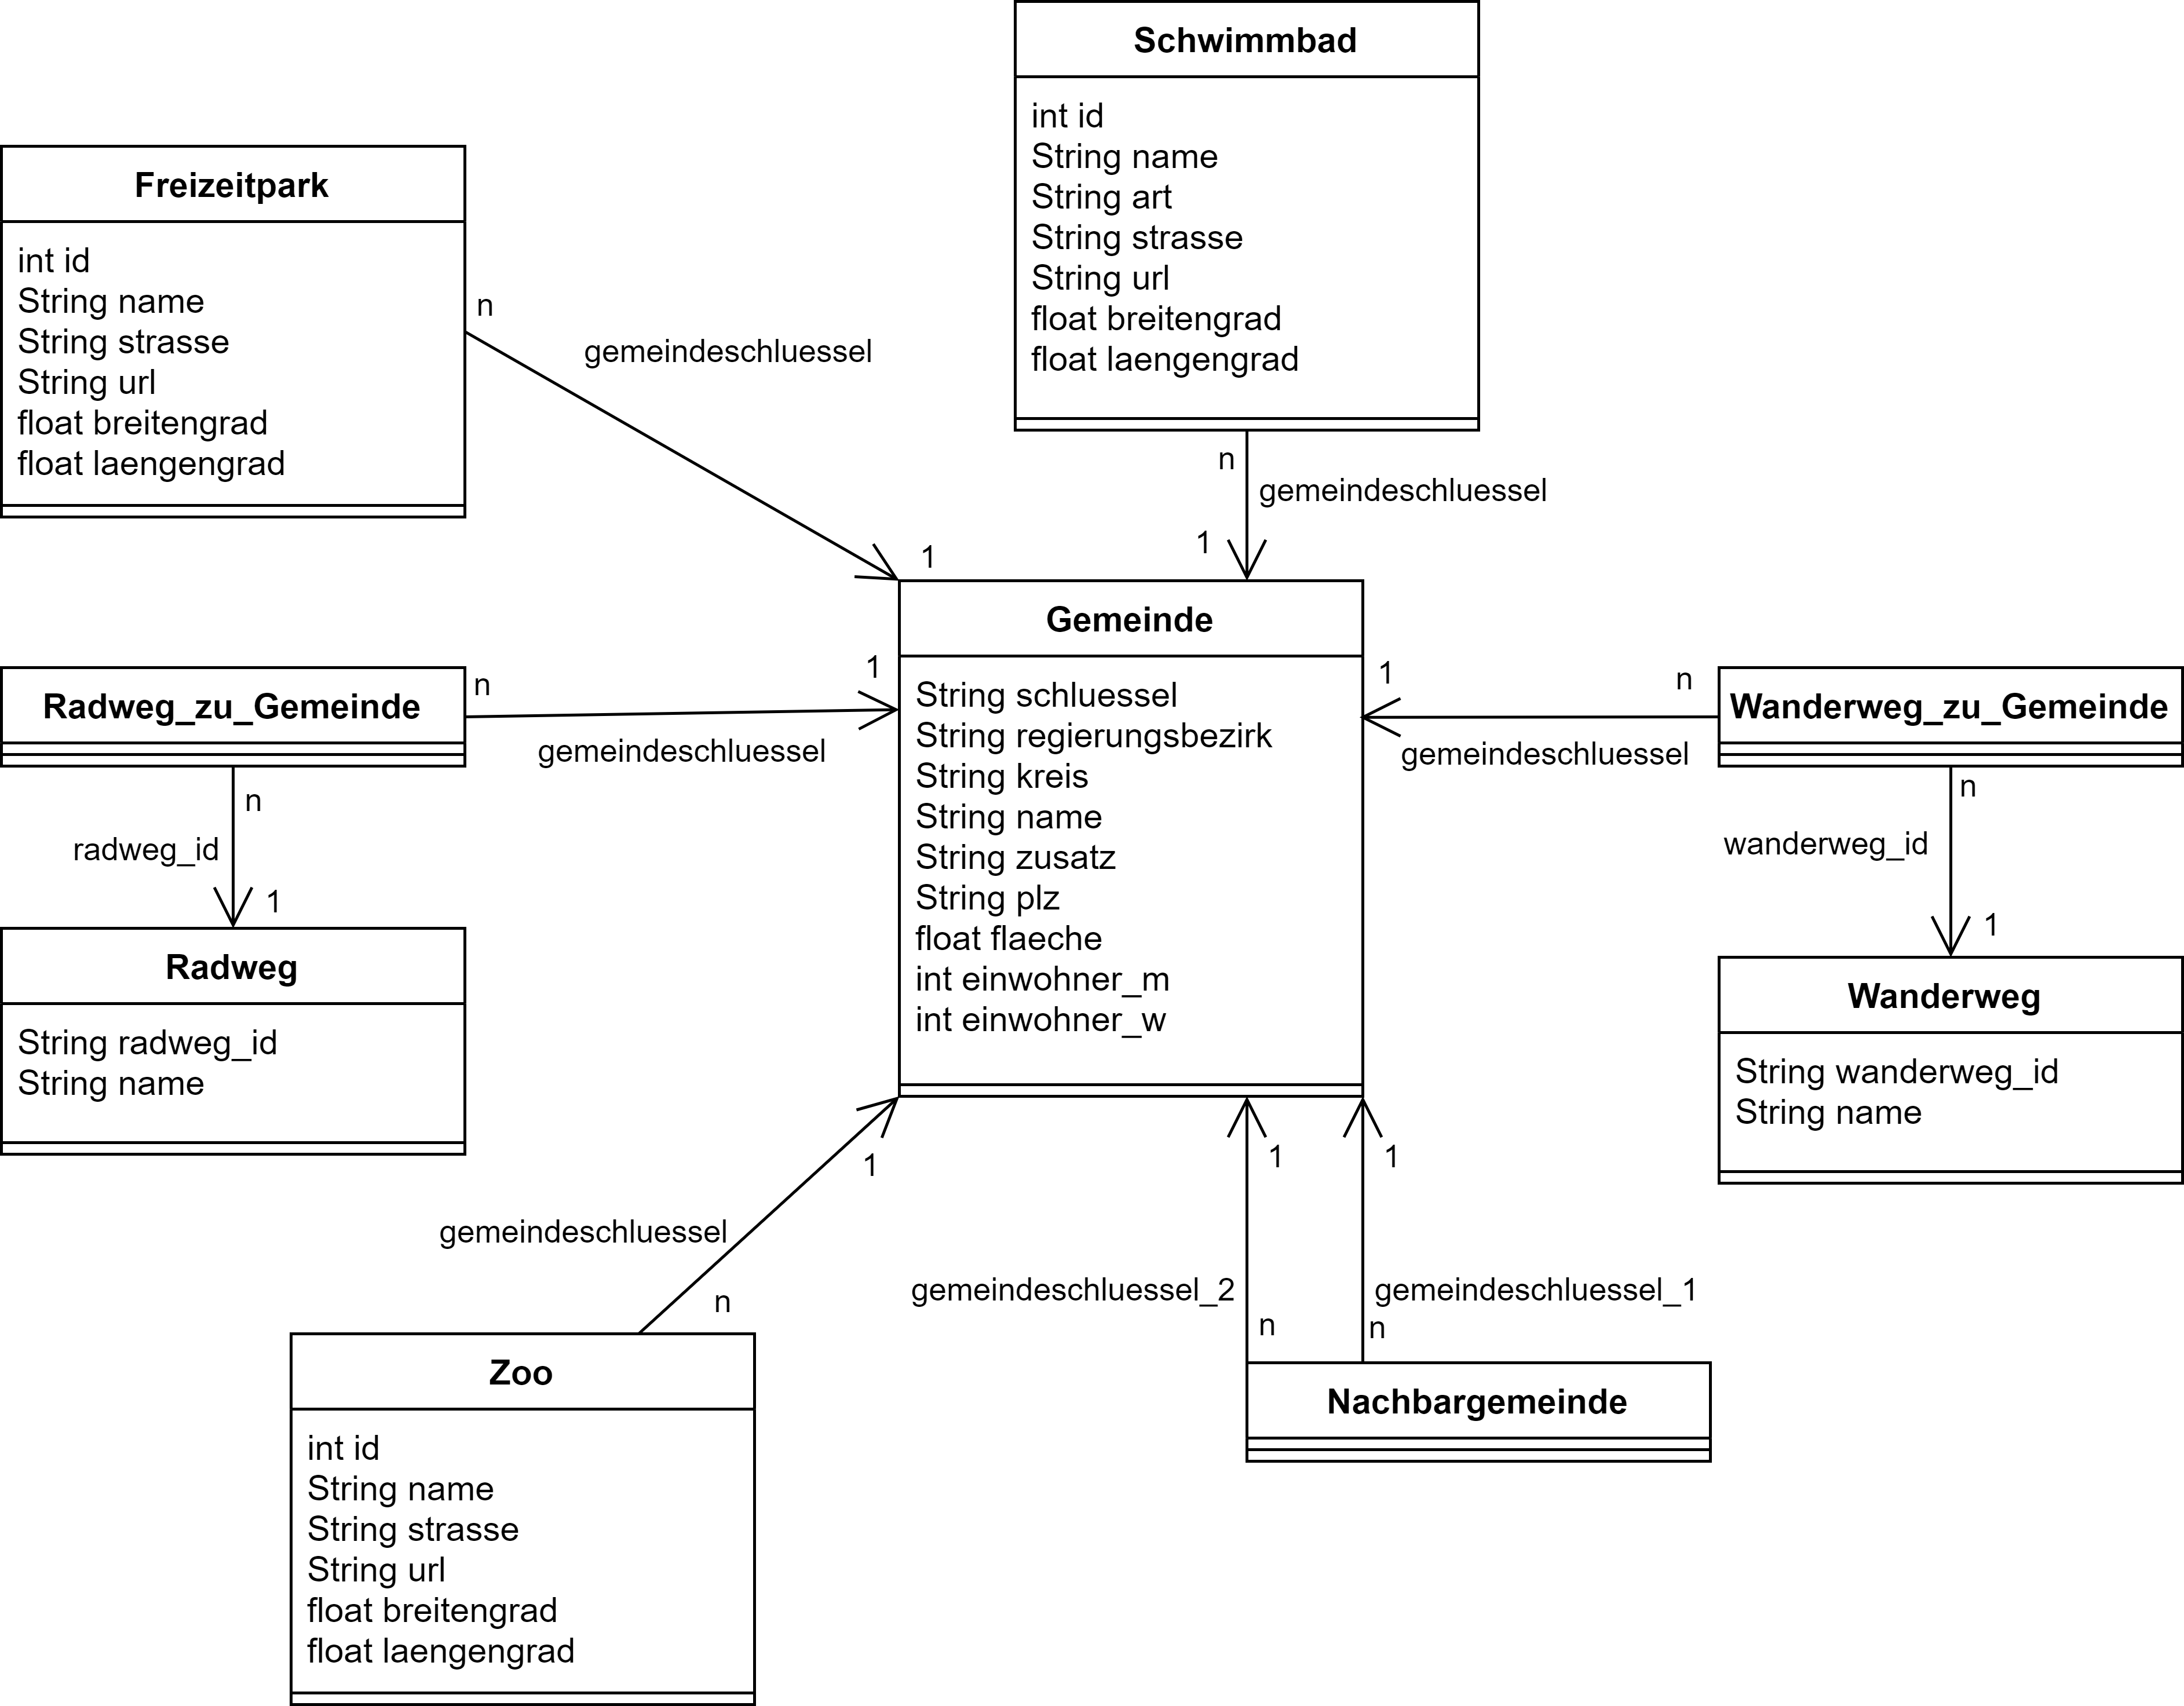
\includegraphics[width=\textwidth]{Aufgaben/img/Bayern_DB.png}}{49}
\end{minipage}